\begin{framed}

Objetivos:
\begin{itemize}
    \item Entender el rol del número de Reynolds en la capa límite.
    \item Analizar la fuerza sobre una placa plana.
    \item Derivar expresiones para el espesor de la capa límite.
\end{itemize}

Contenidos:
\begin{itemize}
    \item El número de Reynolds en capa límite.
    \item La relación integral de momentum en una placa plana.
    \item Placa plana sin gradiente de presión.
    \item El espesor de capa límite de von Kármán.
    \item El espesor de capa límite de Blasius.
\end{itemize}

Bibliografía:
\begin{itemize}
    \item White, F. M. (2008) Mecánica de Fluidos. McGraw-Hill. Sexta edición. Secciones 7.2-7.4
    \item Fox, R. W., Pritchard, P. J. y McDonald, A. T. (2009) Introduction to Fluid Mechanics. John Wiley \& Sons. Secciones 9.4-9.5
\end{itemize}
\end{framed}

\section*{El número de Reynolds}

En el caso del flujo sobre una placa plana que hemos estado discutiendo, la placa se puede considerar infinitamente larga.
Esto nos p[one en una disyuntiva \mbox{?`}cuál es el número de Reynolds que caracteriza al problema entonces?
Resulta que la mejor manera que analizar estos problemas es considerando un número de Reynolds variable en el espacio.
Por lo tanto, para una misma placa plana, tendremos una distribución de números de Reynolds, donde:
%
\begin{equation}\label{eq:Re_capa}
Re_x = \frac{U_\infty x}{\nu}.
\end{equation}

Una implicancia interesante es que si analizamos en una longitud suficientemente larga, siempre vamos a llegar a número de Reynolds suficientemente altos como para empezar a ver turbulencia.
De hecho, como lo muestra la Figura \ref{fig:capa_limite_Re}, esto se ve en la práctica. 
La capa límite sobre una placa plana es siempre laminar inicialmente, y eventualmente se torna turbulenta, agua abajo.
El número de Reynolds crítico en capa límite es alrededor de $5\cdot10^{-5}$.
%
\begin{figure}[!h]
\centering
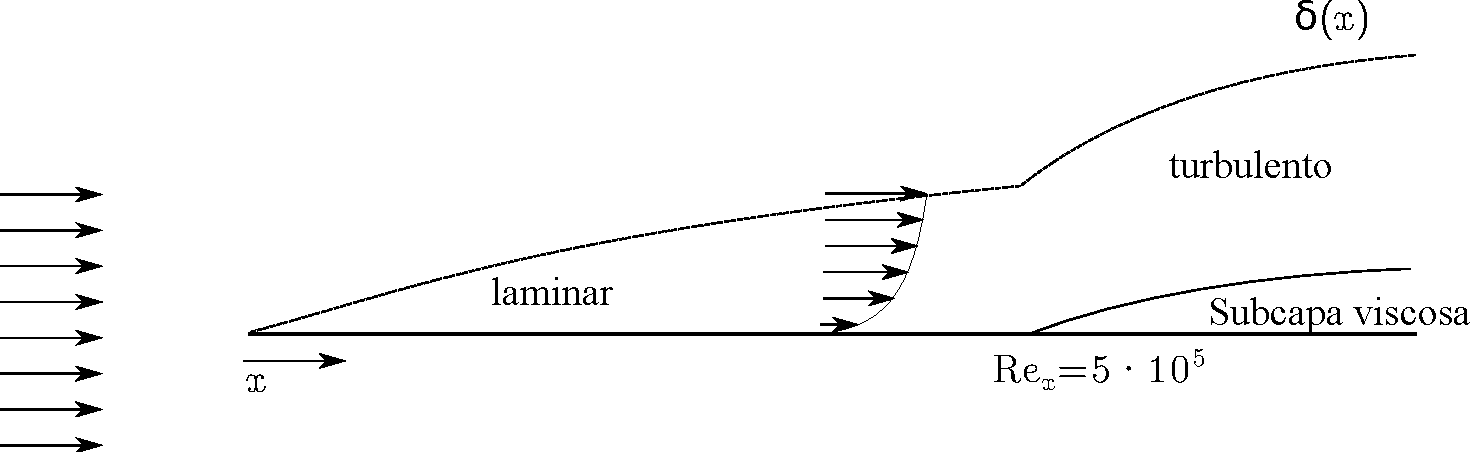
\includegraphics[width=0.8\textwidth]{clase09/capa_limite_Re.pdf}
\caption{Capa límite en función de $Re_x$.}
\label{fig:capa_limite_Re}
\end{figure}

Cuando la capa límite se torna turbulenta, aparece una pequeña zona laminar, pegada a la placa, que se conoce como subcapa viscosa.
Aparte de ser laminar, esta zona tiene importantes implicancias en el patrón del flujo dentro de la capa límite, ya que, si su espesor es mayor que la rugosidad de la placa, esta rugosidad no afecta al flujo y se puede considerar como una placa lisa. 
Como pueden imaginarse, esto tiene un importante efecto en el arrastre sobre la placa.

A continuación veremos algunas soluciones de capa límite, que dependen del número de Reynolds definido en la Ec. \eqref{eq:Re_capa}, tanto para flujo laminar, como para turbulento.

\section*{Espesor de capa límite laminar sin gradiente de presión}

\subsection*{El análisis de von Kármán}
\paragraph*{La relación integral de momentum.}

Quizás la forma más fácil de encontrar una expresión para el espesor de capa límite $\delta$ es a través de un análisis de cantidad de movimiento de la placa.
De hecho, la clase pasada hicimos este análisis para el caso particular en que la velocidad fuera de la capa límite $U_\infty$ sea independiente de $x$, y llegamos a
%
\begin{align}
D(x) &= \rho bU_\infty^2\theta\text{, con el espesor de momentum,}\nonumber\\
\theta &= \int_0^\delta\frac{u(y)}{U_\infty}\left(1-\frac{u(y)}{U_\infty}\right)\mathrm{d}y
\end{align}

De no ser $U_\infty$  independiente de $x$, por Bernoulli podemos darnos cuenta que habría un gradiente de presión, y considerando que $dp/dy=0$ dentro de la capa límite, tendríamos que sumar la contribución de este $\Delta p$ a la suma de fuerzas.
De este caso ya hablaremos más adelante.

La fuerza sobre la placa $D(x)$ es el resultado de esfuerzos cortantes ($\tau_w$) a lo largo de la placa.
Matemáticamente, esto es
%
\begin{equation}
D(x) = b\int_0^x \tau_w(x)\mathrm{d}x,
\end{equation}
%
lo que implica que
%
\begin{align}\label{eq:tau_w}
\frac{dD}{dx}=b\tau_w \text{ y, }\nonumber\\
\tau_w=\rho U_\infty^2 \frac{d\theta}{dx}.
\end{align}
%
Esta última relación se conoce como la relación integral de momentum para flujo en la capa límite sobre una placa plana.

\paragraph*{Espesor de capa límite de von Kármán.}
Para obtener una expresión de $\delta(x)$, von Kármán asumió un perfil de velocidad con forma parabólica:
%
\begin{equation}\label{eq:perfil_vk}
u(x,y) = U_\infty\left(\frac{2y}{\delta}-\frac{y^2}{\delta^2}\right) \quad 0\leq y\leq \delta(x).
\end{equation}
%
Reemplazando la Ec. \eqref{eq:perfil_vk} en el espesor de momentum $\theta$, llegamos a
%
\begin{equation}\label{eq:espesor_mom_vk}
\theta = \int_0^\delta \left(\frac{2y}{\delta} - \frac{y^2}{\delta^2}\right)\left(1-\frac{2y}{\delta} + \frac{y^2}{\delta^2}\right)\mathrm{d}y=\frac{2}{15}\delta.
\end{equation}
%
Podemos también calcular $\tau_w$ usando:
%
\begin{equation}\label{eq:tau_w2}
\tau_w = \mu\frac{du}{dy} = 2\frac{\mu U_\infty}{\delta}.
\end{equation}
%
Reemplazando la relación integral de momentum (Ec. \eqref{eq:tau_w}) en la Ec. \eqref{eq:tau_w2}, y usando la Ec. \eqref{eq:espesor_mom_vk} llegamos a una expresión para $\delta$:
%
\begin{align}
2\frac{\mu U_\infty}{\delta} &= \rho U_\infty^2 \frac{d\theta}{dx} = \rho U_\infty^2 \frac{2}{15}\frac{d\delta}{dx}\nonumber\\
\Rightarrow \delta d\delta &= 15\frac{\nu}{U_\infty}dx
\end{align}
% 
e integrando esta última expresión, tomando en cuenta que $\delta=0$ para $x=0$, obtenemos:
%
\begin{align}\label{eq:delta_vk}
\frac{1}{2}\delta^2 &= 15 \frac{\nu x}{U_\infty} \nonumber\\
\Rightarrow \frac{\delta}{x} &= 5.5\left(\frac{\nu}{U_\infty x}\right)^{1/2} = \frac{5.5}{\sqrt{Re_x}}.
\end{align}
%
Como adelantamos al principio de la clase, obtuvimos una expresión en función de $Re_x$.

Por otra parte, podemos también calcular el coeficiente de arrastre local $c_f$ como:
%
\begin{equation}\label{eq:cf_vk}
c_f = \frac{\tau_w}{\frac{1}{2}\rho U_\infty^2} = 4\frac{1}{\rho U_\infty^2}\frac{\mu U_\infty}{\delta} = \frac{0.73}{\sqrt{Re_x}}
\end{equation}
%
y el espesor de desplazamiento:
%
\begin{align}\label{eq:desplazamiento_vk}
\delta^* &= \int_0^\delta\left(1-\frac{u}{U_\infty}\right)\mathrm{d}y = \int_0^\delta \left(1-\frac{2y}{\delta}+\frac{y^2}{\delta^2}\right)\nonumber\\
&= \left. y-\frac{y^2}{\delta}+\frac{y^3}{3\delta}\right/_0^\delta = \frac{\delta}{3}\nonumber\\
\Rightarrow \frac{\delta^*}{x} &= \frac{1.83}{\sqrt{Re_x}}
\end{align}

Los valores de espesor de capa límite obtenidos con el análisis de von Kármán dependen de la aproximación que la velocidad dentro de la capa límite tiene forma parabólica. 
En la realidad, esto no es así, sin embargo los valores de $\delta$, $\delta^*$, $c_f$, $\tau_w$ y $\theta$ dados por este análisis hacen buenas predicciones y, en general, están a menos de un 10\% del valor real.

\section*{Espesor de capa límite de Blasius}

 La clase pasada derivamos la ecuación de Blasius, que describe el perfil de velocidad dentro de la capa límite sobre una placa plana sin gradiente de presión:
 %
 \begin{align}\label{eq:blasius2}
f'''&+\frac{1}{2}ff''=0\nonumber\\
f'(\eta) &= \frac{u}{U_\infty} \nonumber\\
\eta &= y\left(\frac{U_\infty}{\nu x}\right)^{1/2}\nonumber\\
f(0) &= 0\nonumber\\
f'(0) &= 0\nonumber\\
f'(\infty) &= 1
 \end{align}

 La ecuacion de Blasius es una ecuación diferencial ordinaria que no tiene solución analítica, sin embargo, podemos resolverla numéricamente.
 Si se fijan en el código del repositorio Github,\footnote{\url{https://github.com/cdcooper84/mec220/blob/master/apuntes/clase09/blasius.ipynb}} verán  que resolvemos esta ecuación con un método de Euler, y que el borde de la capa límite (donde $u=0.99U_\infty$), se da para $\eta=5$.
En este punto $y=\delta$, y reemplazando en la Ec. \eqref{eq:blasius2} llegamos a
%
\begin{equation}\label{eq:delta_blasius}
\frac{\delta}{x} = \frac{5}{\sqrt{Re_x}}
\end{equation}

Comparando las Ecs. \eqref{eq:delta_vk} y \eqref{eq:delta_blasius}, nos podemos dar cuenta que la solución dada por von Kármán, que asume un perfil parabólico, no está tan lejos de la solución real.
En el caso de von Kármán, llegamos a un factor $5.5$ y en Blasius de $5$, solamente un 10\% de diferencia.
Además, vemos en la Figura \ref{fig:capa_limite_blasius} que el perfil parabólico de von Kármán (línea punteada) es una buena aproximación del perfil de Blasius (línea sólida) dentro de la capa límite.
%
\begin{figure}
\centering
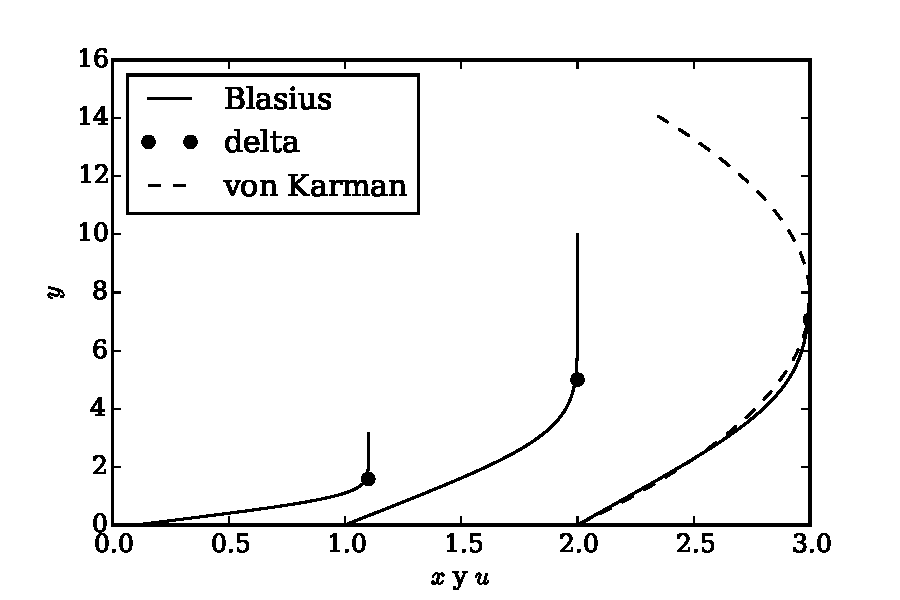
\includegraphics[width=0.7\textwidth]{clase09/capa_limite_blasius.pdf}
\caption{Perfil de velocidad dentro de la capa límite para $x=0.1$, $x=1$ y $x=2$. Línea sólida representa el perfil de Blasius, los puntos sólidos el fin de la capa límite, y la línea punteada el perfil parabólico de von Kármán.}
\label{fig:capa_limite_blasius}
\end{figure}

\paragraph*{Espesor de desplazamiento}

El espesor de desplazamiento de define como 
%
\begin{equation}
\delta^* = \int_0^\infty\left(1-\frac{u(y)}{U_\infty}\right)dy
\end{equation}
%
lo cual podemos reescribir en términos de $f(\eta)$, con $dy = d\eta\left(\frac{\nu x}{U_\infty}\right)^{1/2}$
%
\begin{align}
\delta^* &= \left(\frac{\nu x}{U_\infty}\right)^{1/2}\int_0^\infty(1-f'(\eta))d\eta\\
& = \left.\left(\frac{\nu x}{U_\infty}\right)^{1/2} (\eta-f(\eta))\right|_\infty
\end{align}

Usando el mismo código que antes, nos damos cuenta que al infinito el valor de $\eta-f'(\eta)$ tiende a 1.721, y podemos escribir
%
\begin{equation}
\frac{\delta^*}{x} = \frac{1.721}{\sqrt{Re_x}}
\end{equation}

\paragraph*{Esfuerzo cortante.}
Sabemos que la definición de $\tau_w$ es
%
\begin{equation}
\tau_w = \left.\mu\frac{du}{dy}\right|_0
\end{equation}
%
lo cual se puede escribir en términos de $f$ y $\eta$ como
%
\begin{align}
\tau_w &= \left. U_\infty\mu \frac{df'}{dy}\right|_0 = U_\infty\mu \left(\frac{U_\infty}{\nu x}\right)^{1/2}f''(0) \nonumber\\
&= U_\infty^{3/2}\left(\frac{\mu\rho}{x}\right)^{1/2}f''(0) = 0.332055 U_\infty^{3/2}\left(\frac{\mu\rho}{x}\right)^{1/2} 
\end{align}
%
Por otra parte, el coeficiente de arrastre es
%
\begin{equation}
c_f = \frac{\tau_w}{\frac{1}{2}U_\infty^2\rho} = \frac{2\cdot0.332055}{\sqrt{Re_x}} = \frac{0.664}{\sqrt{Re_x}}
\end{equation}

\paragraph*{Espesor de momentum.}
En la definición del espesor de momentum dijimos que
%
\begin{equation}
\tau_w = \rho U_\infty^2 \frac{d\theta}{dx}
\end{equation}
%
y usando la expresión que encontramos recién para $\tau_w$, quedamos con
%
\begin{align}
\theta &= \int_0^x 0.332 U_\infty^{3/2}\left(\frac{\mu\rho}{x}\right)^{1/2} \frac{1}{\rho U_\infty^2} dx \nonumber\\
&= \int_0^x 0.332 \left(\frac{\mu}{xU_\infty\rho}\right)^{1/2} dx = 2\cdot0.332 x^{1/2}\left(\frac{\mu}{U_\infty\rho}\right)^{1/2}
\end{align}
%
y dividiendo por $x$, queda
%
\begin{equation}
\frac{\theta}{x} = \frac{0.664}{\sqrt{Re_x}}
\end{equation}
